%----------------------------------------------------------------
%
%  File    :  survey-SVG.tex
%
%  Author  : Alexei Kruglov, TU Graz, Austria
% 
%  Created :  01 Dec 2016
% 
%  Changed :  X Dec 2016
% 
%----------------------------------------------------------------


\section{Scalable Vector Graphics (SVG)}
\label{sect:SVG}
%\TODO{{section by A.K.}}
SVG (Scalable Vector Graphics) is an XML (Extensible Markup Language) based specification for describing two-dimensional graphics in a vector form. It is specified by W3C (World Wide Web Consortium). Initial release was made in 2001, and the latest release (1.1) was in 2011. Currently it is used in all latest major web browsers, such as Google Chrome, Mozilla Firefox and Internet Explorer, and in some vector graphics software editors, as Inkscape and Adobe Illustrator. In contrast to raster images, vector images are resolution independent, as the format itself is lossless. As mentioned before, the graphic is described in an XML textual file, which can be compressed with gzip. As a result of compression, web pages, where SVG is used load faster than those which use standard JPEG or PNG graphics solutions. Because graphics can be directly embedded into HTML, no extra HTTP requests are necessary. Above approaches lead to saving of the bandwidth, which is extremely important on the pages with higher loads. SVG has a support for different graphics effects and animations, which can be further enhanced with CSS and JavaScript. In case SVG graphic is made in a very complex node structure, browser can have problems rendering the image. In this case other technologies can be used. SVG integrates with other W3C standards such as the DOM and XSL\citep{w3schoolSVG}. 

\subsection{SVG basic graphical elements} % (fold)
\label{sub:SVG_basic_elemnts}
As mentioned before SVG graphics can be embedded directly into HTML pages
\begin{lstlisting}[
language=CSS,
label=list:BibACMIEEE,
caption={[Example of SVG embedded directyl into HTML]%
Simple example code one circle embedded directyl into HTML.
}
]
<html>
<body>

<svg width="100" height="100">
  <circle cx="50" cy="50" r="40" stroke="green" stroke-width="4" fill="yellow" />
</svg>

</body>
</html>

\end{lstlisting}
\label{list:SVGHTML}
\begin{figure}[h]
\centering
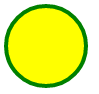
\includegraphics[keepaspectratio,scale=0.5]{images/circle.png}

\caption[SVG basic graphical elements]{
This example shows how simple to add one element (circle) embedded directyl into HTML. 
\imgcredit{Screenshot taken by the authors of this survey. The code behind the pages is by using the \citet{CircleHtml} online snippets as a base.}

}
\label{fig:circleHTML}
\end{figure}
SVG consists of different basic graphical elements, from which more complex elements can be derived. Basic elements included in SVG are:
\begin{description}
\item [<rect>] 	  -Element is used to draw a rectangle and variations of the shape of a rectangle.
\item [<circle>]      	 -Element is used to create a simple circle with color options.
\item [<line>]         	 -Element is used to create a line.
\item [<polygon>]  	 -Element is used to create a graphic that contains at least three sides.
\item [<polyline>]  	 -Element is used to provide any shape consisting of straight lines.
\item [<path>]    	 -Element is used to define a path. Participates in paths drawing strongly to use to encourage the SVG editor to create complex graphics.
\end{description}

With these simple, basic of elements, you can build a very complex shapes. With heli additional graphics functions, you can create a moving figures, but if these figures create just only SVG, the program code will be very large and difficult to read.
\begin{figure}[h]
\centering
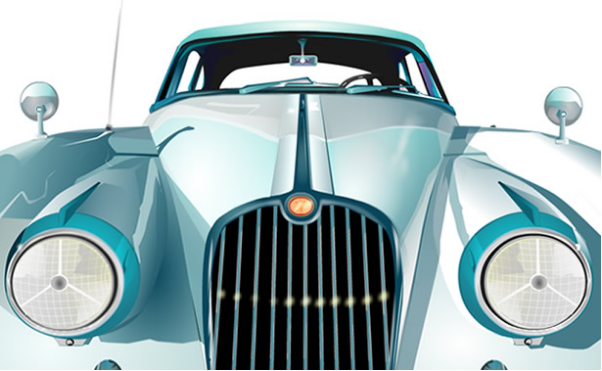
\includegraphics[keepaspectratio,scale=0.5]{images/Car_svg.png}

\caption[Complex picture with simple SVG elements]{
Example to create one complex picture with simple SVG elements, with help geomety and color options.
\imgcredit{Screenshot taken by the authors of this survey. The code behind the pages is by using the \citet{CarSVGl} online snippets as a base.}

}
\label{fig:Circle_HTML}
\end{figure}
% SVG basic graphical elements (end)
\subsection{SVG animation } % (fold)
SVG element is a specific DOM element, which includes himself syntax standard HTML-element. SVG elements have unique tags, attributes and behaviors that enable them to determine any form that offer the opportunity to essentially produce directly to the DOM, images, and thereby benefit from the JavaScript and CSS-based manipulation. There are three main advantages to create graphics in SVG, than an image (PNG, JPEG, etc.): First, compresses incredibly well, certain terms in the SVG file format is smaller than their PNG / JPEG equivalents. Secondly, SVG graphics to scale to any resolution without loss of clarity; they look sharp on all desktop and mobile screens. Third, you can animate the individual components of the SVG graphics performance (with help JavaScript and CSS).SVG elements take some of the standard CSS properties, but not all. In addition, SVG takes a certain set of "presentation" attributes, such as fill, x and y, which also serve to determine both the SVG is visually observed. There is no functional difference between the SVG specification of style using CSS, or as an attribute - SVG specification only divide property under two. In following examples shows how SVG work with CSS together:
\begin{description}
\item [Define the imeage as vectors in SVG]
\item [Tranform the vectors with CSS or SVG]
\end{description}
\begin{lstlisting}[
language=CSS,
label=list:BibACMIEEE,
caption={[Define the imeage as vectors in SVG]%
Define the attribute for animate transorm.
}
]
<animateTransform attributeName="transform"
		attributeType="XML"
		type="translate"
		values="0 50;0 -50;"
		dur="2s"
		repeatCount="indefinite"/>

\end{lstlisting}
\label{list:animateTransorm}
\subsubsection {Create SVG stucture into HTML} % (fold)
\begin{lstlisting}[
language=CSS,
label=list:BibACMIEEE,
caption={[Create SVG stucture into HTML]%
Define svg class  with three simple {\em{}<path>} SVG elements with transform function .
}
]
<svg class="svg-icon" viewBox="0 0 20 20">
		<path id="svg-doc" d="M15.475,6.692l-4.084-4.083C11.32,
		2.538,11.223,2.5,11.125,2.5h-6c-0.413,0-0.75,0.337-0.75,
		0.75v13.5c0,0.412,0.337,0.75,0.75,0.75h9.75c0.412,
		0,0.75-0.338,0.75-0.75V6.94C15.609,6.839,15.554,6.771,
		15.475,6.692 M11.5,3.779l2.843,2.846H11.5V3.779z
		M14.875,16.75h-9.75V3.25h5.625V7c0,0.206,0.168,0.375,
		0.375,0.375h3.75V16.75z"
		transform="scale(0.25) translate(27.5)"></path>

		<path id="svg-bottom" fill="none" d="M16.471,
		5.962c-0.365-0.066-0.709,0.176-0.774,0.538l-1.843,
		10.217H6.096L4.255,6.5c-0.066-0.362-0.42-0.603-0.775-0.538
		C3.117,6.027,2.876,6.375,2.942,6.737l1.94,10.765c0.058,
		0.318,0.334,0.549,0.657,0.549h8.872c0.323,0,0.6-0.23,
		0.656-0.549l1.941-10.765C17.074,6.375,16.833,6.027,16.471,
		5.962z"
		transform="scale(0.75) translate(4,20)"></path>

		<path id="svg-deck" fill="none" d="M16.594,3.804H3.406
		c-0.369,0-0.667,0.298-0.667,0.667s0.299,0.667,0.667,
		0.667h13.188c0.369,0,0.667-0.298,0.667-0.667S16.963,
		3.804,16.594,3.804zM9.25,3.284h1.501c0.368,0,0.667-0.298,
		0.667-0.667c0-0.369-0.299-0.667-0.667-0.667H9.25c-0.369,
		0-0.667,0.298-0.667,0.667C8.583,2.985,8.882,3.284,9.25,3.284z"
		transform="scale(0.75) translate(4,20)"></path>
	</svg>

\end{lstlisting}
\label{list:SVGStuctureHTML}

\subsubsection {Define keyframe in CSS} % (fold)
\begin{lstlisting}[
language=CSS,
label=list:BibACMIEEE,
caption={[Create Keys CSS]%
Create CSS with {\em{@keyframes}} for picture visualization  .
}
]
#svg-doc{
	fill:red;
	animation: doc-delete 4s linear infinite;
}

#svg-deck{
	transform-origin: 100% 50%;
	animation: deck-rot 4s linear infinite;
}

@keyframes doc-delete {
	0% { transform: translate(75%) scale(0.25); }
	15% { transform: translate(75%) scale(0.25); }
	65% { transform: translate(85%,150%) scale(0.1) rotate(-180deg);}
	100% { transform: translate(85%,150%) scale(0.1); opacity: 0;}
}

@keyframes deck-rot {
	0% { transform: translate(-9%, 440%) rotate(0deg) scale(0.75); }
	25% { transform: translate(-9%, 440%) rotate(90deg) scale(0.75);}
	40% { transform: translate(-9%, 440%) rotate(90deg) scale(0.75);}
	65% { transform: translate(-9%, 440%) rotate(0deg) scale(0.75);}
	100% { transform: translate(-9%, 440%) rotate(0deg) scale(0.75);}

\end{lstlisting}
\label{list:Keys_CSS}

\begin{figure}[h]
\centering

\includegraphics[keepaspectratio,scale=0.5]{images/beer_svg.png}

\caption[Complete example create animation SVG with CSS]{
Example to create one complex moving animation in SVG with help of CSS.
\imgcredit{Screenshot taken by the authors of this survey. The code behind the pages is by using the \citet{beerSVG} online snippets as a base.}

}
\label{fig:SVG_CSS}
\end{figure}


\begin{figure}[h]
\centering

\includegraphics[keepaspectratio,scale=0.5]{images/icon_svg.png}

\caption[Animation from finished icons]{
Example to create animation with help prepared simple icons. 
\imgcredit{Screenshot taken by the authors of this survey. The code behind the pages is by using the \citet{trashSVG} online snippets as a base.}

}
\label{fig:SVGWithSimpleIcons}
\end{figure}